
\definecolor{ce6e6e6}{RGB}{230,230,230}
\definecolor{cff0000}{RGB}{255,0,0}
\definecolor{c00ff00}{RGB}{0,255,0}
\definecolor{c0000ff}{RGB}{0,0,255}
\definecolor{cffffff}{RGB}{255,255,255}


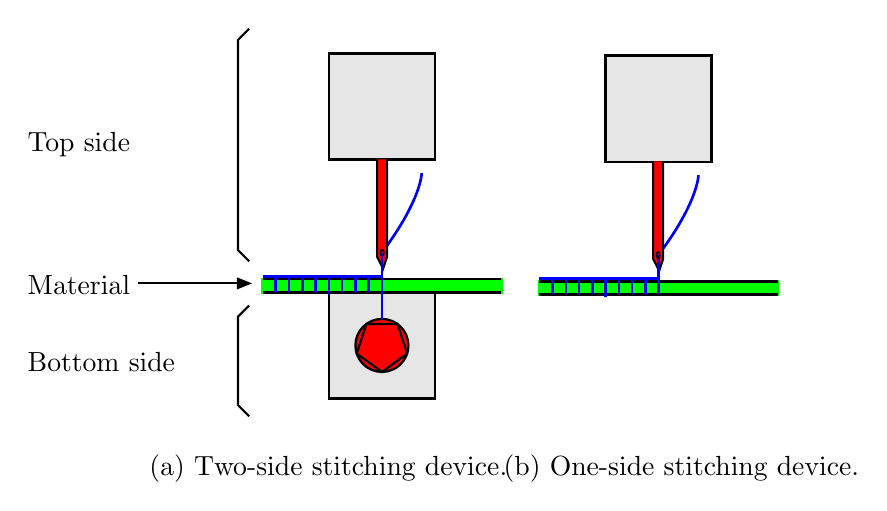
\begin{tikzpicture}[y=0.80pt, x=0.8pt,yscale=-1, inner sep=0pt, outer sep=0pt]
\begin{scope}[shift={(0,-308.26769)}]
  \path[draw=black,fill=ce6e6e6,miter limit=4.00,line width=0.958pt,rounded
    corners=0.0000cm] (191.0420,461.4252) rectangle (238.9580,509.3412);
  \path[cm={{1.1979,0.0,0.0,1.1979,(155.105,266.93151)}},draw=black,fill=cff0000,miter
    limit=4.00,line width=0.800pt]
    (60.0000,182.3622)arc(0.000:180.000:10.000)arc(-180.000:0.000:10.000) --
    cycle;
  \path[cm={{1.1979,0.0,0.0,1.1979,(161.0945,266.93151)}},draw=black,fill=cff0000,miter
    limit=4.00,line width=0.800pt] (45.0000,192.3622) -- (35.4894,185.4523) --
    (39.1221,174.2720) -- (50.8779,174.2720) -- (54.5106,185.4523) -- cycle;
  \path[draw=black,fill=ce6e6e6,miter limit=4.00,line width=0.958pt,rounded
    corners=0.0000cm] (191.0420,353.6142) rectangle (238.9580,401.5302);
  \path[draw=c00ff00,fill=c00ff00,miter limit=4.00,line width=0.958pt,rounded
    corners=0.0000cm] (161.0945,455.4357) rectangle (268.9055,461.4252);
  \path[draw=black,line join=miter,line cap=butt,line width=0.958pt]
    (161.0945,461.4252) -- (268.9055,461.4252);
  \path[draw=black,fill=c0000ff,line join=miter,line cap=butt,line width=0.958pt]
    (268.9055,455.4357) -- (161.0945,455.4357);
  \path[draw=c0000ff,line join=miter,line cap=butt,line width=0.958pt]
    (215.0000,443.4567) .. controls (232.9685,419.4987) and (232.9685,407.5197) ..
    (232.9685,407.5197);
  \path[draw=black,fill=cff0000,line join=miter,line cap=butt,line width=0.720pt]
    (212.8580,401.3142) -- (212.8580,445.4142) -- (215.5580,450.8142) --
    (217.3580,445.4142) -- (217.3580,401.3142);
  \path[cm={{1.44946,0.0,0.0,1.44946,(-92.90204,263.74434)}},draw=black,fill=cffffff,line
    join=round,miter limit=4.00,fill opacity=0.011,line width=0.601pt]
    (213.0000,124.0945)arc(0.000:180.000:0.500000 and
    1.000)arc(-180.000:0.000:0.500000 and 1.000) -- cycle;
  \path[draw=c0000ff,line join=miter,line cap=butt,line width=0.958pt]
    (161.0945,454.2378) -- (167.0840,454.2378) -- (167.0840,461.4252) --
    (167.0840,454.2378) -- (173.0735,454.2378) -- (173.0735,461.4252) --
    (173.0735,454.2378) -- (179.0630,454.2378) -- (179.0630,461.4252) --
    (179.0630,454.2378) -- (185.0525,454.2378) -- (185.0525,461.4252) --
    (185.0525,454.2378) -- (191.0420,454.2378) -- (191.0420,462.6231) --
    (191.0420,454.2378) -- (197.0315,454.2378) -- (197.0315,461.4252) --
    (197.0315,454.2378) -- (203.0210,454.2378) -- (203.0210,461.4252) --
    (203.0210,454.2378) -- (209.0105,454.2378) -- (209.0105,461.4252) --
    (209.0105,454.2378) -- (215.0000,454.2378) -- (215.0000,461.4252) --
    (215.0000,443.4567);
  \path[draw=c0000ff,line join=miter,line cap=butt,line width=0.958pt]
    (215.0000,461.4252) -- (215.0000,473.4042);
  \path[draw=black,fill=ce6e6e6,miter limit=4.00,line width=0.958pt,rounded
    corners=0.0000cm] (316.0420,354.5512) rectangle (363.9580,402.4672);
  \path[draw=c00ff00,fill=c00ff00,miter limit=4.00,line width=0.958pt,rounded
    corners=0.0000cm] (286.0945,456.3727) rectangle (393.9055,462.3622);
  \path[draw=black,line join=miter,line cap=butt,line width=0.958pt]
    (286.0945,462.3622) -- (393.9055,462.3622);
  \path[draw=black,fill=c0000ff,line join=miter,line cap=butt,line width=0.958pt]
    (393.9055,456.3727) -- (286.0945,456.3727);
  \path[draw=c0000ff,line join=miter,line cap=butt,line width=0.958pt]
    (340.0000,444.3937) .. controls (357.9685,420.4357) and (357.9685,408.4567) ..
    (357.9685,408.4567);
  \path[draw=black,fill=cff0000,line join=miter,line cap=butt,line width=0.720pt]
    (337.5205,402.2512) -- (337.5205,446.3512) -- (340.2205,451.7512) --
    (342.0205,446.3512) -- (342.0205,402.2512);
  \path[draw=c0000ff,line join=miter,line cap=butt,line width=0.958pt]
    (286.0945,455.1748) -- (292.0840,455.1748) -- (292.0840,462.3622) --
    (292.0840,455.1748) -- (298.0735,455.1748) -- (298.0735,462.3622) --
    (298.0735,455.1748) -- (304.0630,455.1748) -- (304.0630,462.3622) --
    (304.0630,455.1748) -- (310.0525,455.1748) -- (310.0525,462.3622) --
    (310.0525,455.1748) -- (316.0420,455.1748) -- (316.0420,463.5601) --
    (316.0420,455.1748) -- (322.0315,455.1748) -- (322.0315,462.3622) --
    (322.0315,455.1748) -- (328.0210,455.1748) -- (328.0210,462.3622) --
    (328.0210,455.1748) -- (334.0105,455.1748) -- (334.0105,462.3622) --
    (334.0105,455.1748) -- (340.0000,455.1748) -- (340.0000,462.3622) --
    (340.0000,444.3937);
  \path[fill=black] (110,547.36218) node[above right] (text3003) {(a) Two-side
    stitching device.};
  \path[fill=black] (270,547.36218) node[above right] (text3007) {(b) One-side
    stitching device.};
  \path[shift={(0,308.26769)},draw=black,line join=miter,line cap=butt,line
    width=0.800pt] (155.0000,149.0945) -- (105.0000,149.0945);
  \path[shift={(0,308.26769)},draw=black,fill=black,line join=miter,line
    cap=butt,line width=0.800pt] (155.0000,149.0945) -- (150.0000,147.0945) --
    (150.0000,151.0945) -- cycle;
  \path[shift={(0,308.26769)},draw=black,line join=miter,line cap=butt,line
    width=0.800pt] (155.0000,139.0945) -- (150.0000,134.0945) --
    (150.0000,39.0945) -- (155.0000,34.0945);
  \path[shift={(0,308.26769)},draw=black,line join=miter,line cap=butt,line
    width=0.800pt] (155.0000,159.0945) -- (150.0000,164.0945) --
    (150.0000,204.0945) -- (155.0000,209.0945);
  \path[fill=black] (55,462.36218) node[above right] (text3023) {Material};
  \path[fill=black] (55,400.36218) node[above right] (text3027) {Top side};
  \path[fill=black] (55,497.36218) node[above right] (text3031) {Bottom side};
  \path[cm={{1.44946,0.0,0.0,1.44946,(31.76047,264.68134)}},draw=black,fill=cffffff,line
    join=round,miter limit=4.00,fill opacity=0.011,line width=0.601pt]
    (213.0000,124.0945)arc(0.000:180.000:0.500000 and
    1.000)arc(-180.000:0.000:0.500000 and 1.000) -- cycle;

\end{scope}

\end{tikzpicture}

